\documentclass[11pt,a4paper]{article}
\usepackage[utf8]{inputenc}
\usepackage[T1]{fontenc}
\usepackage{amsmath,amssymb}
\usepackage{graphicx}
\usepackage{xcolor}
\usepackage{hyperref}
\usepackage{geometry}
\usepackage{tikz}
\usepackage{enumitem}
\usepackage{float}
\usepackage{caption}
\usepackage{booktabs}

\geometry{margin=2.0cm,columnsep=0.7cm}
\usetikzlibrary{arrows.meta,positioning,fit,backgrounds,calc}
\hypersetup{colorlinks=true,linkcolor=blue,urlcolor=blue,citecolor=blue}
\definecolor{primary}{RGB}{41,128,185}
\definecolor{success}{RGB}{39,174,96}
\definecolor{accent}{RGB}{211,84,0}
\definecolor{darkgray}{RGB}{44,62,80}
\definecolor{lightgray}{RGB}{245,247,250}

\title{\textbf{Weekly Report}\\[4pt]\large Qlab-Oriented SDCS Small-Map Planning\\and 2D Vehicle-Following Controller Design}
\author{Qi LI}
\date{July 31, 2026}

\begin{document}
\setcounter{tocdepth}{1}
\twocolumn[
\maketitle
\tableofcontents
\vspace{.3em}
]
\small

\section{Work summary}
This week has two connected parts:
\begin{itemize}[leftmargin=*]
    \item \textbf{SDCS small-map planning baseline:} transferred the Qlab-oriented roadmap and smooth-turn approach into the current QCar/CARLA project, then checked the resulting route in CARLA.
\item \textbf{2D vehicle-following controller design:} formulated the Chapter~3 look-ahead controller for the QCar bicycle model and identified the remaining observer and steering constraints.
\end{itemize}

The CARLA result in this report is a path-planning and path-following baseline. The 2D platoon controller and distributed high-gain observer are still design work and are not claimed as validated results.

\section{SDCS planner: Qlab-to-project baseline}

\subsection{Reference and transfer objective}
The SDCS small-map planner was oriented from the Qlab path-planning reference. The reference provides the roadmap and smooth-turn idea; the project version brings this idea into the current QCar/CARLA environment as a self-contained planner for the SDCS small map.

\begin{figure}[H]
\centering
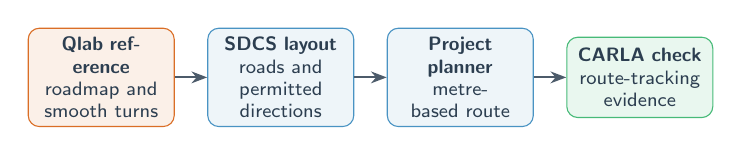
\begin{tikzpicture}[
  font=\sffamily\scriptsize,
  source/.style={rectangle,rounded corners=4pt,draw=accent!85,fill=accent!9,text=darkgray,align=center,text width=1.62cm,minimum height=1.02cm},
  stage/.style={rectangle,rounded corners=4pt,draw=primary!85,fill=primary!8,text=darkgray,align=center,text width=1.62cm,minimum height=1.02cm},
  result/.style={rectangle,rounded corners=4pt,draw=success!85,fill=success!10,text=darkgray,align=center,text width=1.62cm,minimum height=1.02cm},
  arrow/.style={-{Stealth[length=2mm]},draw=darkgray!85,line width=.8pt}
]
\node[source] (qlab) at (0,0) {\textbf{Qlab reference}\\roadmap and smooth turns};
\node[stage] (map) at (2.28,0) {\textbf{SDCS layout}\\roads and permitted directions};
\node[stage] (project) at (4.56,0) {\textbf{Project planner}\\metre-based route};
\node[result] (carla) at (6.84,0) {\textbf{CARLA check}\\route-tracking evidence};
\draw[arrow] (qlab) -- (map);
\draw[arrow] (map) -- (project);
\draw[arrow] (project) -- (carla);
\end{tikzpicture}
\caption{Transfer path from the Qlab planning reference to the project-local SDCS small-map baseline.}
\label{fig:qlab-transfer}
\end{figure}

\subsection{What was retained and adapted}
\begin{table}[H]
\centering\tiny
\setlength{\tabcolsep}{2pt}
\begin{tabular}{@{}p{1.3cm}p{3.1cm}p{3.1cm}@{}}
\toprule
\textbf{Aspect} & \textbf{Qlab reference} & \textbf{Current project planner}\\
\midrule
Purpose & General roadmap support for Quanser environments. & Route generation for the SDCS small map used by QCar/CARLA.\\
Road layout & A reusable map structure made of locations and road connections. & Eleven fixed small-map locations with permitted directed connections.\\
Route choice & A valid shortest connection between requested locations. & A valid right-hand-traffic route through requested small-map locations.\\
Path shape & Straight sections and smooth turns. & The same route-shape idea, sampled as tracking waypoints.\\
Execution environment & Uses the Qlab support environment. & Runs inside this project without requiring the licensed Qlab library at runtime.\\
Evidence & Reference implementation. & CARLA route-tracking artifact in Figure~\ref{fig:sdcs-baseline}.\\
\bottomrule
\end{tabular}
\caption{Comparison between the Qlab reference and the project-local SDCS planner.}
\label{tab:qlab-comparison}
\end{table}

\subsection{Planner outcome and current integration}
The planner receives a requested sequence of map locations, connects them through permitted roads, and returns a smooth waypoint route. A route can end at its requested destination or repeat as a closed circuit. This gives the control system a repeatable path reference for CARLA tests.

\begin{figure}[H]
\centering
\resizebox{.98\columnwidth}{!}{%
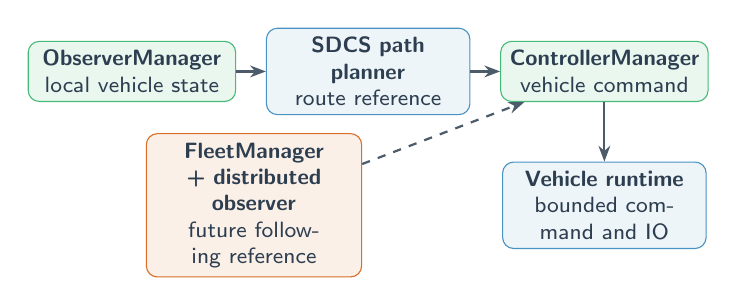
\begin{tikzpicture}[
  font=\sffamily\footnotesize,
  module/.style={rectangle,rounded corners=4pt,draw=primary!85,fill=primary!8,text=darkgray,align=center,text width=2.35cm,minimum height=.73cm},
  manager/.style={rectangle,rounded corners=4pt,draw=success!85,fill=success!10,text=darkgray,align=center,text width=2.4cm,minimum height=.73cm},
  future/.style={rectangle,rounded corners=4pt,draw=accent!85,fill=accent!9,text=darkgray,align=center,text width=2.5cm,minimum height=.73cm},
  arrow/.style={-{Stealth[length=2mm]},draw=darkgray!85,line width=.8pt},
  dashedarrow/.style={arrow,dashed}
]
\node[manager] (observer) at (-2.55,1.15) {\textbf{ObserverManager}\\local vehicle state};
\node[module] (planner) at (.45,1.15) {\textbf{SDCS path planner}\\route reference};
\node[manager] (controller) at (3.45,1.15) {\textbf{ControllerManager}\\vehicle command};
\node[future] (fleet) at (-1.0,-.55) {\textbf{FleetManager + distributed observer}\\future following reference};
\node[module] (vehicle) at (3.45,-.55) {\textbf{Vehicle runtime}\\bounded command and IO};
\draw[arrow] (observer) -- (planner);
\draw[arrow] (planner) -- (controller);
\draw[arrow] (controller) -- (vehicle);
\draw[dashedarrow] (fleet) -- (controller);
\end{tikzpicture}}
\caption{Current SDCS path-reference flow and the future fleet-following integration point.}
\label{fig:planner-integration}
\end{figure}

\begin{figure}[H]
\centering
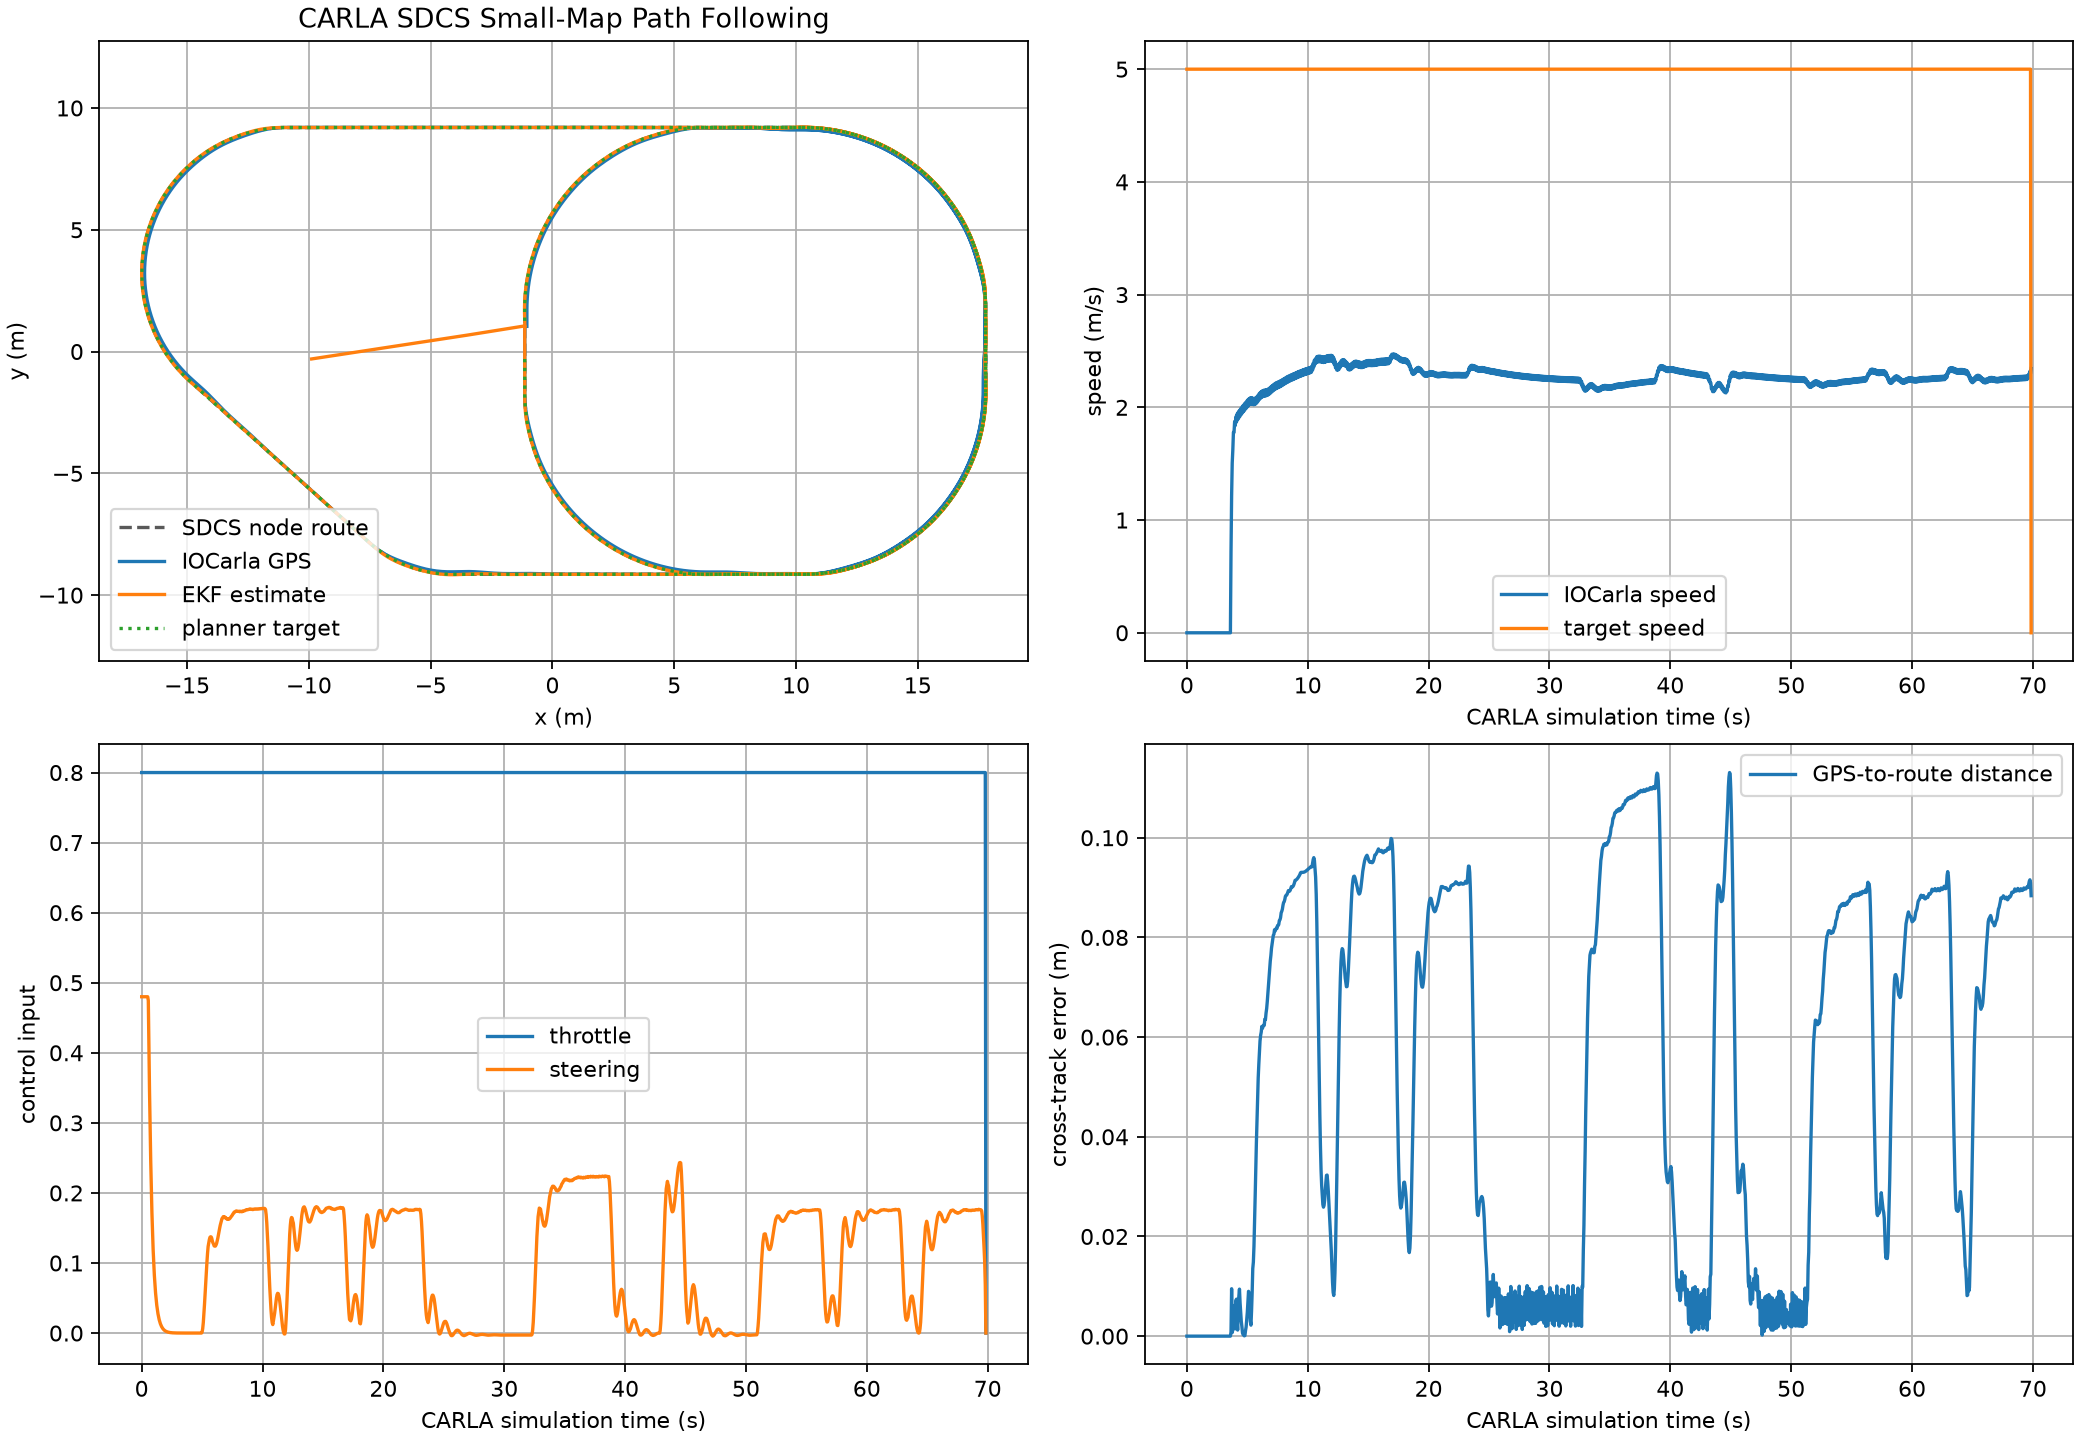
\includegraphics[width=\columnwidth]{../../test/artifacts/integration_carla_sdcs_path.png}
\caption{Quanser SDCS map trajectory following under CARLA with ego vehicle. The planner target, estimated path, speed, commands, and cross-track error are recorded for review.}
\label{fig:sdcs-baseline}
\end{figure}

\section{2D following-control formulation}

\subsection{Reference model and time-gap objective}
The following formulation is based on Chapter~3 of Bayuwindra's PhD thesis on look-ahead tracking controllers for integrated longitudinal and lateral vehicle-platoon control.\footnote{A.~Bayuwindra, \emph{Look-ahead tracking controllers for integrated longitudinal and lateral control of vehicle platoons}, PhD thesis, Eindhoven University of Technology, 2019, Chapter~3.}

For vehicle $i$, the reference model is
\begin{equation}
\dot{x}_i=v_i\cos\psi_i,\ 
\dot{y}_i=v_i\sin\psi_i,\ 
\dot{v}_i=a_i,\ 
\dot{\psi}_i=\omega_i,
\label{eq:unicycle-model}
\end{equation}
with
\begin{equation}
u_i^{\mathrm{ref}}=
\begin{bmatrix}a_i&\omega_i\end{bmatrix}^{\top}.
\label{eq:unicycle-input}
\end{equation}

\begin{equation}
\begin{aligned}
p_i&=\begin{bmatrix}x_i&y_i\end{bmatrix}^{\top},\\
d_{r,i}&=(r_i+h_iv_i)
\begin{bmatrix}\cos\psi_i\\\sin\psi_i\end{bmatrix},
\end{aligned}
\label{eq:time-gap-distance}
\end{equation}
\begin{equation}
e_i=(p_{i-1}-p_i)-d_{r,i}.
\label{eq:spacing-error}
\end{equation}

\subsection{Error-state feedback form}
Error Dynamics:
\begin{equation}
z_i=
\begin{bmatrix}
e_{x,i}\\ e_{y,i}\\
v_{i-1}\cos\psi_{i-1}-v_i\cos\psi_i\\
v_{i-1}\sin\psi_{i-1}-v_i\sin\psi_i
\end{bmatrix}.
\label{eq:error-state}
\end{equation}

Control input:
\begin{equation}
\begin{bmatrix}a_i\\\omega_i\end{bmatrix}
=F_i^{-1}
\begin{bmatrix}
z_{3,i}+k_{1,i}z_{1,i}\\
z_{4,i}+k_{2,i}z_{2,i}
\end{bmatrix},
\label{eq:chapter-three-feedback}
\end{equation}
where $k_{1,i}$ and $k_{2,i}$ are controller parameters, and
\begin{equation}
F_i=
\begin{bmatrix}
h_i\cos\psi_i & -(r_i+h_iv_i)\sin\psi_i\\
h_i\sin\psi_i & \phantom{-}(r_i+h_iv_i)\cos\psi_i
\end{bmatrix}.
\label{eq:unicycle-feedback-matrix}
\end{equation}
{\it Remark: Note that the control input is for 2 wheel unicycle vehicles. So the yaw rate $\omega_i$ is directly commanded, which is not the case for 4 wheel vehicles. The bicycle model transformation is needed to convert the yaw-rate command into a front-wheel steering command.}
\subsection{Bicycle-model transformation}
For 4 wheel vehicle $i$ is a bicycle model with wheelbase $L$ and front-wheel steering $\delta_{f,i}$. The bicycle model is transformed into the unicycle form in \eqref{eq:unicycle-model} by
\begin{equation}
\begin{aligned}
\dot{\psi}_i&=\frac{v_i}{L}\tan\delta_{f,i},\qquad
\kappa_i=\frac{1}{L}\tan\delta_{f,i},\\
\omega_i&=v_i\kappa_i.
\end{aligned}
\label{eq:bicycle-yaw}
\end{equation}
\begin{equation}
\begin{bmatrix}\ddot{x}_i\\\ddot{y}_i\end{bmatrix}
=
\underbrace{\begin{bmatrix}
\cos\psi_i & -v_i^2\sin\psi_i\\
\sin\psi_i & \phantom{-}v_i^2\cos\psi_i
\end{bmatrix}}_{H_i}
\begin{bmatrix}a_i\\\kappa_i\end{bmatrix}.
\label{eq:bicycle-acceleration}
\end{equation}
\begin{equation}
F_i^{\mathrm{bike}}=
\begin{bmatrix}
h_i\cos\psi_i & -v_i(r_i+h_iv_i)\sin\psi_i\\
h_i\sin\psi_i & \phantom{-}v_i(r_i+h_iv_i)\cos\psi_i
\end{bmatrix},
\label{eq:bicycle-feedback-matrix}
\end{equation}
\begin{equation}
\begin{bmatrix}a_i\\\kappa_i\end{bmatrix}
=\left(F_i^{\mathrm{bike}}\right)^{-1}
\begin{bmatrix}
z_{3,i}+k_{1,i}z_{1,i}\\
z_{4,i}+k_{2,i}z_{2,i}
\end{bmatrix}.
\label{eq:bicycle-feedback}
\end{equation}
\begin{equation}
\delta_{f,i}=\arctan(L\kappa_i).
\label{eq:steering-conversion}
\end{equation}

\subsection{Next step: Observable-form target and constraints}
- Triangular-form representation of controlled platoon model:
\begin{equation}
\zeta_i=T(q_i)=
\begin{bmatrix}
X_i&\dot{X}_i&\ddot{X}_i&Y_i&\dot{Y}_i&\ddot{Y}_i
\end{bmatrix}^{\top}.
\label{eq:coordinate-target}
\end{equation}
\begin{equation}
\begin{aligned}
\dot{\zeta}_{i,j}&=\zeta_{i,j+1},\\
\dot{\zeta}_{i,r}&=\varphi_i(\zeta_i,u_i)+d_i,\qquad
y_i=C\zeta_i.
\end{aligned}
\label{eq:triangular-target}
\end{equation}
\begin{equation}
\boxed{\begin{gathered}
T(\cdot),\ \varphi_i(\cdot),\ \text{and }y_i\\
\text{remain to be derived.}
\end{gathered}}
\label{eq:observer-open}
\end{equation}
- The constraints on the bicycle model: steering angle $\delta_{f,i}$ is bounded, for qcar $\delta_{\max}=\frac{1}{6}\pi$~rad.
\begin{equation}
\boxed{\begin{gathered}
\psi_i\notin u_i^{\mathrm{bike}},\qquad
\delta_{f,i}\in[-\delta_{\max},\delta_{\max}],\\
\delta_{f,i}^{\star}=\arctan\!\left(\frac{L\omega_i^{\star}}{v_i}\right),\qquad v_i>0.
\end{gathered}}
\label{eq:steering-constraints}
\end{equation}

{\footnotesize
\begin{itemize}[leftmargin=*,topsep=1pt,itemsep=1pt,parsep=0pt]
    \item \textit{Observer form:} derive $T(\cdot)$ and $y_i$ for an observable canonical or triangular form.
    \item \textit{Yaw and steering:} yaw is reached only indirectly through limited steering; the yaw-rate-to-steering conversion is unsuitable near zero speed.
\end{itemize}}

\end{document}
